\documentclass[11pt,a4paper]{article}
\usepackage[margin=2.2cm]{geometry}
\usepackage[T1]{fontenc}
\usepackage[utf8]{inputenc}
\usepackage{lmodern}
\usepackage{graphicx}
\usepackage{booktabs}
\usepackage{tabularx}
\usepackage{multirow}
\usepackage{amsmath}
\usepackage{xcolor}
\usepackage{enumitem}
\usepackage[colorlinks=true,linkcolor=blue!50!black,urlcolor=blue!50!black,citecolor=blue!50!black]{hyperref}

\setlist{itemsep=2pt,topsep=3pt}
\newcommand{\Rtoa}{R_\mathrm{toa}}
\newcommand{\Rrs}{R_\mathrm{rs}}
\newcommand{\code}[1]{\texttt{#1}}
\newcommand{\todo}[1]{\textcolor{red!70!black}{[#1]}}
\newcommand{\prio}[1]{\textbf{\textcolor{blue!50!black}{#1}}}

\title{RadCalNet-OC: validation, performance and roadmap}
\author{Tristan Harmel}
\date{Draft --- November 2026}

\begin{document}
\maketitle

\begin{abstract}
\code{radcalnet\_oc} propagates the water-leaving reflectance measured by AERONET-OC stations to the top of
the atmosphere (TOA) for the Cal/Val of optical satellite sensors over water. This draft reports
(i)~the first systematic Sentinel-2/MSI L1C validation at four AERONET-OC sites (535 clear matchups),
(ii)~the theoretical validation of the gaseous absorption--scattering coupling against SOS-ABS simulations,
(iii)~the computing performance of the chain, and (iv)~a prioritised roadmap. In the visible, the simulated
TOA reflectance agrees with MSI within $-3$ to $0\,\%$ (443--560\,nm). Beyond 665\,nm the simulation is
systematically too low by $2$--$3\times10^{-3}$ in reflectance, nearly flat with wavelength, i.e.\ $-8\,\%$
at 705\,nm to $-60\,\%$ at 2190\,nm in relative terms. This deficit decreases with the angular distance to
the specular direction and increases with the aerosol optical thickness, which points first to the sunglint
and to the aerosol model as the priorities of the roadmap.
\end{abstract}

\tableofcontents

%=====================================================================================================
\section{Scope and status of the package}
%=====================================================================================================

The TOA reflectance is simulated with the gaseous absorption coupled with the scattering: the path
reflectance and the water-leaving term have their own gaseous transmittances,
\begin{equation}
\Rtoa(\lambda) = \pi\, \Rrs(\lambda)\, T^{\downarrow}(\lambda)\, t^{\uparrow}(\lambda)\, T_g^{w}(\lambda)
+ T_g^{atm}(\lambda)\, R_\mathrm{atm}(\lambda)
+ T_{dir}(\lambda)\, R_{sg},
\label{eq:rtoa}
\end{equation}
where the last term is the direct sunglint: $R_{sg}$ is the Cox--Munk reflectance of the direct sunlight by the
wind-roughened surface (with wave shadowing), attenuated by the direct transmittance of the
Sun-surface-sensor path, $T_{dir}(\lambda) = T_g(\lambda, m)\, \exp[-(\tau_r(\lambda)+\tau_a(\lambda))\, m]$
with $m = 1/\mu_0+1/\mu_v$. The look-up tables contain only the diffuse light, so this term is computed
separately (\code{coxmunk.Sunglint}) and added for the comparisons with the satellite (Sec.~\ref{sec:matchups}).
The gaseous transmittances of the path reflectance, the water-leaving term and the irradiance,
$X\in\{atm, w, E_d\}$, are given by a photon path-length model (Gamma distribution of the absorber
paths, equivalence theorem),
\begin{equation}
T_g^{X}(\lambda) = \left(1 + s_X^2\, \eta_X\, \tau_g(\lambda, m_X)\right)^{-1/s_X^2},
\qquad \tau_g(\lambda, m) = -\ln T_g(\lambda, m),
\label{eq:ppld}
\end{equation}
where $T_g(\lambda, m)$ is the direct-beam gaseous transmittance (REPTRAN, line-by-line for O$_2$) for the
geometric air mass $m_{atm}=m_w=1/\mu_0+1/\mu_v$ or $m_{E_d}=1/\mu_0$, and $\eta_X$ (mean absorber path relative
to the geometric one) and $s_X^2$ (its relative variance) are fitted per absorption window and term on full
radiative transfer simulations of the coupled absorption and scattering (SOS-ABS), as functions of the air
mass, the AOT and the water vapour column. The path reflectance sees only a fraction of the geometric path
($\eta_{atm}\approx0.45$--$0.65$ in 684--990\,nm), the water-leaving term and the irradiance slightly more
($\eta\approx1.02$--$1.05$). The downwelling irradiance is $E_d = T^{\downarrow}\, T_g^{E_d}\, E_0$.

For $\eta_X=1$ and $s_X^2\to0$, all terms see the direct beam, $T_g^{atm}=T_g^{w}=T_g^{\downarrow}T_g^{\uparrow}$,
and the first two terms of Eq.~\eqref{eq:rtoa} reduce to the factorised form of the versions before 1.1,
$\Rtoa = T_g^{\downarrow} T_g^{\uparrow}\left[\pi\,\Rrs\,T^{\downarrow}t^{\uparrow} + R_\mathrm{atm}\right]$, which
underestimates the band TOA reflectance by about 4\,\% (O$_2$-B), 10--15\,\% (720, 820, 900\,nm), 30\,\%
(O$_2$-A head) and 50--60\,\% (940\,nm). The coupled model is the default in the H$_2$O and O$_2$ windows of
684--990\,nm; elsewhere (and for O$_3$, NO$_2$, CH$_4$) $T_g^X = T_g(\lambda, m_X)$, its extension to
350--2500\,nm being part of the roadmap.

$R_\mathrm{atm}$ (Rayleigh, aerosol and sky reflection by the wind-roughened surface) comes from the
GRS radiative transfer look-up table (\code{toa\_lut\_opac\_wind\_v3.nc}, Zenodo
\href{https://doi.org/10.5281/zenodo.23394202}{10.5281/zenodo.23394202}) and the transmittances
$T^{\downarrow}$, $t^{\uparrow}$ from the companion transmittance LUT. The simulation is hyperspectral
(350--2500\,nm) and convolved with the sensor spectral responses.

\paragraph{Grid of the TOA LUT.} 6 OPAC aerosol models (ARCT, COAV, DESE, MACL, URBA at 70\,\% RH, WASO dry),
10 reference AOT nodes (0--1.5), 6 wind speeds (0.5--16\,m\,s$^{-1}$), 45 solar zenith angles (0--88$^\circ$),
34 viewing zenith angles (0--48.9$^\circ$), 73 relative azimuths (5$^\circ$ step) and only
\textbf{10 wavelength nodes} (350, 400, 500, 600, 700, 800, 1000, 1600, 2200, 2500\,nm), between which the
path reflectance is interpolated.

\paragraph{Released and unreleased features.} Version 1.0.2 is on PyPI. The \code{[Unreleased]} section of the
changelog holds major changes now in the defaults of the development branch:
line-by-line O$_2$ (\code{o2\_model='lbl'}), the photon path-length model of the gas--scattering coupling
in 684--990\,nm (\code{gas\_coupling='path\_length'}), wind speed as an input interpolated between the LUT
nodes, the spectral extension of $\Rrs$ beyond the input range (pure water + fitted particulate
backscattering), the hyperspectral reconstruction of the multispectral AERONET-OC $\Rrs$ with invRrs, tabulated
spectral responses (\code{Spectral.from\_srf}) and the access to AERONET-OC through the shared
\code{aeronet\_oc\_db} database.

%=====================================================================================================
\section{Validation}
%=====================================================================================================

\subsection{Theoretical validation: gaseous absorption coupled with scattering}

The decoupled model applies the gaseous transmittance of the direct beam to all the terms. Against SOS-ABS
coupled simulations (CKD 5\,cm$^{-1}$, maritime aerosols, US62, H$_2$O 0.5--4\,g\,cm$^{-2}$, SZA 20--70$^\circ$,
AOT(550) 0.05--0.4; 678 absorbing channels in 19 windows over 350--2500\,nm):

\begin{itemize}
\item the path reflectance sees only a fraction of the geometric air mass: $\eta_\mathrm{atm}=0.41$ (940\,nm) to
  0.87 (2150\,nm) in median for H$_2$O, 0.48 (O$_2$-A) to 0.89 (CH$_4$ 2300\,nm) for the well-mixed gases; O$_3$
  ($\eta\approx1.00$) and CO$_2$ 1600\,nm ($\eta\approx1.04$) are already well described by the decoupled model;
\item decoupled error of the band path reflectance (absorption-depth error): 45--48\,\% for OLCI Oa19/Oa20 and
  MSI B9, 29--34\,\% for the cirrus bands (MSI B10, OLI B9), 21--29\,\% for Oa13/Oa15/Oa21, 6--13\,\% in the SWIR;
  water-leaving term and irradiance only 0.1--0.6\,\%;
\item the photon path-length (Gamma distribution) model, one model per window and term, reduces these errors to
  6--8\,\% (Oa19, Oa20, B9), 5--6\,\% (cirrus bands), 2--5\,\% (Oa13, Oa15); the residual band TOA error of the path
  reflectance is 4.6--6.1\,\% in the 940\,nm and cirrus bands and $<1\,\%$ elsewhere. It extrapolates in water
  vapour and geometry (leave-one-out: $\le0.5$ point).
\end{itemize}

The path-length model is the default in 684--990\,nm only. Beyond 990\,nm the package is still decoupled, and
the absorption tables themselves differ by more than the coupling residual in several windows (REPTRAN vs
CKD: $+25$--40\,\% in H$_2$O 720/900/1880/2150\,nm, $-33\,\%$ in H$_2$O 1380\,nm).

\subsection{Sentinel-2/MSI L1C matchups at the TOA}
\label{sec:matchups}

\paragraph{Protocol} (\code{scripts/s2\_toa\_matchup/s2\_toa\_matchup.py}).
For each L1C subset around an AERONET-OC site with AERONET-OC data within $\pm2$\,h of the overpass:
\begin{enumerate}
\item \emph{satellite}: median TOA reflectance in a $1.2\times1.2$\,km box centred on the site, over the pixels
  with finite values in all bands, B10 (1375\,nm) $<0.01$ and B11 (1610\,nm) $<0.03$ (\code{sat\_*}); a second set
  without the SWIR threshold keeps the glinted pixels (\code{satg\_*}); mean solar and viewing geometry;
\item \emph{in situ}: AERONET-OC (\code{aeronet\_oc\_db}) water vapour, ozone, NO$_2$, pressure, wind, spectral AOT;
  hyperspectral $\Rrs$ reconstructed at nadir with invRrs (350--1150\,nm) and extended to 2500\,nm (pure water);
\item \emph{simulation}: \code{radcalnet\_oc} for each measurement of the window at the geometry of the overpass,
  with the aerosol mixture (DESE/MACL/WASO) retrieved from the spectral AOT (\code{kernel.Aerosol}),
  band-integrated with the MSI spectral responses weighted by $E_0$; the direct sunglint, absent from the LUT,
  is added from isotropic Cox--Munk statistics at the AERONET-OC wind speed (\code{simg\_*}).
\end{enumerate}

\paragraph{Data set.} Four site/level combinations are used here (Table~\ref{tab:s2}): AAOT (tile 32TQR,
L2.0 2017-10 to 2025-07 and L1.5 2025-07 to 2026-10), Galata Platform (35TNH, L2.0 2017--2023) and Section-7
Platform (35TPK, L1.5 2024--2026). Lucinda (L1.5: 7 matchups, L2.0: none) and Section-7 L2.0 (3) are too
small to be used. Of the 487 AAOT L2.0 scenes with in situ data, 213 had no valid pixel and 22 had a subset
cut around another site.

\paragraph{Selection.} Valid fraction of the box $>0.5$, $\ge50$ valid pixels, nearest measurement within
60\,min, AOT(550) $<0.3$ and, for the reference statistics, \textbf{glint angle $>30^\circ$} (angle between the
viewing direction and the specular reflection of the Sun), where the simulated direct glint is
$<10^{-3}$ at 865\,nm.

\begin{table}[h]
\centering\small
\caption{Median relative difference (sim $-$ sat)/sat in \%, simulation without direct glint,
glint angle $>30^\circ$. Second line of each site: median absolute difference ($\times10^{-3}$).
B10 (1375\,nm): simulated $\sim10^{-7}$ against $8\times10^{-4}$ observed ($-100\,\%$).}
\label{tab:s2}
\setlength{\tabcolsep}{3pt}
\begin{tabular}{lr*{12}{r}}
\toprule
Site (level) & N & 443 & 490 & 560 & 665 & 705 & 740 & 783 & 842 & 865 & 945 & 1610 & 2190 \\
\midrule
AAOT (L2.0)      & 314 & $-3.0$ & $-0.6$ & $-0.1$ & $-3.9$ & $-7.9$ & $-9.0$ & $-13.0$ & $-14.2$ & $-16.3$ & $-20.5$ & $-39.1$ & $-59.2$ \\
                 &     & $-4.2$ & $-0.6$ & $-0.1$ & $-1.4$ & $-2.2$ & $-2.2$ & $-2.7$ & $-2.5$ & $-2.7$ & $-1.4$ & $-1.8$ & $-1.5$ \\
Galata (L2.0)    &  98 & $-3.0$ & $-1.8$ & $-1.1$ & $-5.8$ & $-8.3$ & $-9.1$ & $-12.6$ & $-13.8$ & $-17.3$ & $-18.0$ & $-45.6$ & $-63.2$ \\
                 &     & $-3.9$ & $-1.7$ & $-0.7$ & $-1.9$ & $-2.7$ & $-2.3$ & $-3.0$ & $-2.5$ & $-2.8$ & $-1.3$ & $-2.5$ & $-2.2$ \\
AAOT (L1.5)      &  99 & $-3.3$ & $-1.4$ & $-1.8$ & $-5.6$ & $-10.0$ & $-11.4$ & $-15.2$ & $-18.5$ & $-20.8$ & $-23.0$ & $-51.3$ & $-67.4$ \\
                 &     & $-4.7$ & $-1.3$ & $-1.2$ & $-1.8$ & $-2.7$ & $-2.6$ & $-3.0$ & $-2.8$ & $-3.2$ & $-1.5$ & $-2.5$ & $-1.9$ \\
Section-7 (L1.5) &  24 & $-4.2$ & $-3.3$ & $-5.6$ & $-13.0$ & $-17.3$ & $-19.1$ & $-22.4$ & $-23.5$ & $-28.4$ & $-29.3$ & $-61.8$ & $-74.6$ \\
                 &     & $-4.9$ & $-3.0$ & $-3.5$ & $-4.7$ & $-5.5$ & $-5.7$ & $-6.3$ & $-5.5$ & $-7.0$ & $-2.3$ & $-5.8$ & $-5.4$ \\
\bottomrule
\end{tabular}
\end{table}

\begin{figure}[h]
\centering
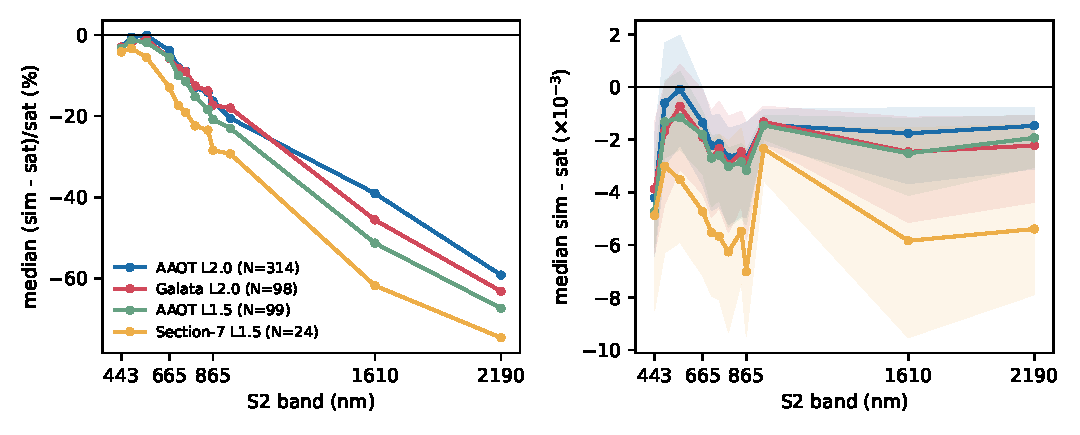
\includegraphics[width=\textwidth]{figures/s2_bias_spectrum.pdf}
\caption{Spectral median difference between the simulation and MSI L1C (glint angle $>30^\circ$, B10 omitted).
Left: relative; right: absolute, with the interquartile range.}
\label{fig:bias}
\end{figure}

\paragraph{Main findings.}
\begin{enumerate}
\item \textbf{Visible: good agreement.} $-3$ to $0\,\%$ at 490--560\,nm at the three main sites; $-3$ to $-4\,\%$
  at 443\,nm ($-4\times10^{-3}$), which is largest for clean atmospheres (AAOT, AOT $<0.08$: $-5.4\times10^{-3}$;
  AOT 0.15--0.3: $-1.8\times10^{-3}$), suggesting a Rayleigh/pressure, blue $\Rrs$ or viewing-geometry
  ($\Rrs$ at nadir) term rather than aerosols.
\item \textbf{NIR--SWIR: systematic deficit of $2$--$3\times10^{-3}$}, nearly flat from 705 to 2190\,nm
  (Fig.~\ref{fig:bias}, right), hence a relative error growing with wavelength as the signal decreases. The same
  shape at all sites points to a common missing contribution rather than to a band-specific gas or calibration
  error. It is larger at Section-7, although this platform is the farthest from the coast (29\,km, against 13\,km
  for AAOT and 23\,km for Galata), and it is mostly an AOT-independent term that vanishes for glint angles
  $>60^\circ$ (Section~\ref{sec:sixs}).
\item \textbf{Dependence on the glint angle.} At AAOT, the deficit at 865\,nm is $-4.0$, $-3.4$, $-2.1$ and
  $-1.1\times10^{-3}$ for glint angles of 30--40, 40--50, 50--60 and $>60^\circ$ (Galata: $-5.4$ to $-1.2$);
  2190\,nm behaves the same (Fig.~\ref{fig:glint}). With MSI near nadir, the glint angle is strongly correlated
  with the solar zenith angle (Spearman $\rho\approx0.5$ for both), so a far glint tail cannot yet be separated
  from an SZA-dependent diffuse term.
\item \textbf{Dependence on the aerosol load.} The NIR--SWIR deficit increases with AOT (AAOT, 2190\,nm:
  $-0.8$, $-1.5$, $-2.2\times10^{-3}$ for AOT $<0.08$, 0.08--0.15, 0.15--0.3). The AOT-proportional part is
  spectrally flat ($-9$ to $-11\times10^{-3}$ per unit AOT from 865 to 2190\,nm) and larger for coarse aerosols
  (Section~\ref{sec:sixs}), consistent with an aerosol model too spectrally steep (coarse mode underestimated)
  in the retrieved DESE/MACL/WASO mixture, and with the coarse spectral sampling of the LUT (1000, 1600,
  2200\,nm nodes); it accounts for about $-1\times10^{-3}$ at a typical AOT of 0.1, i.e.\ a third of the
  deficit.
\item \textbf{Direct sunglint.} Adding the Cox--Munk direct glint reduces the median bias at 865\,nm (all glint
  angles) from $-17.0$ to $-13.5\,\%$ (AAOT L2.0), $-24.9$ to $-6.1\,\%$ (Galata) and $-44.5$ to $0.0\,\%$
  (Section-7 L1.5), but the scatter increases below $30^\circ$ (isotropic statistics, no wind direction, wind
  from the station).
\item \textbf{Cirrus band B10.} Simulated $\sim10^{-7}$ against $8\times10^{-4}$ observed at all sites: the
  saturated H$_2$O band is decoupled beyond 990\,nm, and the observed level may also include stratospheric
  aerosols or the L1C noise floor \todo{to investigate}.
\item \textbf{Sensor units.} At AAOT L2.0, S2A and S2B agree within 1--2 points; S2C matchups (11 at AAOT L2.0,
  28 at AAOT L1.5) are 2--5 points more negative in the NIR--SWIR. Not significant yet (few S2C matchups,
  different period and processing level).
\end{enumerate}

\begin{figure}[h]
\centering
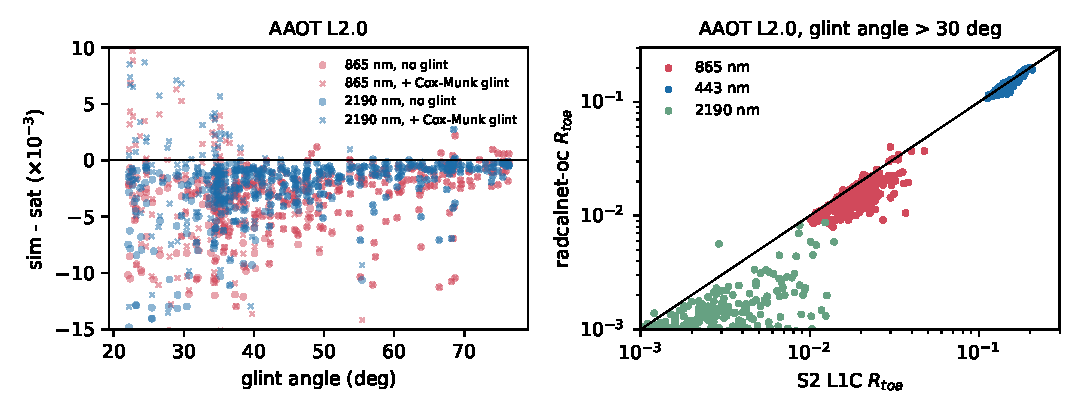
\includegraphics[width=\textwidth]{figures/s2_glint_scatter.pdf}
\caption{AAOT L2.0. Left: difference at 865 and 2190\,nm versus the glint angle, without (dots) and with (crosses)
the simulated direct glint. Right: simulated versus observed TOA reflectance for glint angles $>30^\circ$.}
\label{fig:glint}
\end{figure}

\subsubsection{The NIR--SWIR deficit in view of 6S}
\label{sec:sixs}
The 6S formulation (Vermote et al., \emph{6S User Guide}, version 3, 2006, Part~1, Eqs.~4--8 and 23--26; Part~2,
subroutine ENVIRO) gives a checklist of the terms coupling the atmosphere and the surface: the target contribution
split into direct--direct, diffuse--direct, direct--diffuse and multiple interactions (spherical albedo $S$,
trapping $1/(1-S\rho)$), and, for a non-uniform surface, the environment (adjacency) term
$T(\theta_s)\,t_d(\theta_v)\,\langle\rho\rangle/(1-S\langle\rho\rangle)$. Each one was confronted with the deficit
(\code{scripts/s2\_toa\_matchup/sixs\_terms.py}, same selection as Table~\ref{tab:s2}, AAOT L2.0, AAOT L1.5 and
Galata pooled, $N=511$).

\begin{itemize}
\item \textbf{Surface--atmosphere coupling of the sea surface: already in the LUT.} In the SOS core of OSOAA used for
  the LUT, the direct solar beam reflected by the waves is introduced as a source of the first order of scattering
  and only this direct--direct term (6S Eq.~23) is subtracted from the upward field at the end: the skylight
  reflected by the surface (Eq.~24), the scattering of the reflected direct beam (Eq.~25) and the multiple
  interactions through the spherical albedo (Eq.~26) are in $R_\mathrm{atm}$, and the direct--direct glint is
  added back by the matchup script.
\item \textbf{Trapping of the water signal: negligible.} $T T S\rho_w^2/(1-S\rho_w)$ is below $10^{-5}$ for
  $\rho_w = \pi\Rrs < 0.01$ (NIR--SWIR), and $4\times10^{-4}$ at most for $\rho_w = 0.05$ and $S=0.15$.
\item \textbf{Environment (adjacency) of the coast: one order of magnitude too small and not flat.} With the 6S
  environment functions of the molecules, $F_R(r) = 1-[0.930\,e^{-0.08r}+0.070\,e^{-1.10r}]$, and of the aerosols,
  $F_P(r) = 1-[0.448\,e^{-0.27r}+0.552\,e^{-2.83r}]$ ($r$ in km), the Natural Earth land polygons and the
  reflectance of vegetated land (0.30, 0.22, 0.12 at 865, 1610, 2190\,nm, an upper bound), the term is
  0.22, 0.016, $0.003\times10^{-3}$ at AAOT (coast at 13\,km), 0.10, 0.007, $0.001\times10^{-3}$ at Galata (23\,km)
  and 0.04, 0.002, $0.0004\times10^{-3}$ at Section-7 (29\,km), against $-2.7$, $-1.8$, $-1.5\times10^{-3}$ at
  AAOT. Beyond 10\,km only the molecular environment function contributes: the term collapses in the SWIR and does
  not depend on the aerosol load.
\item \textbf{Whitecaps (Lambertian, absent from OSOAA): not supported.} With the coverage
  $W = 2.95\times10^{-6}U^{3.52}$ and a foam reflectance of 0.22 decreasing in the infrared, they would give
  0.24 (6\,m\,s$^{-1}$) to $0.66\times10^{-3}$ (8\,m\,s$^{-1}$) at 865\,nm, but the deficit does not increase with
  the wind speed (it is even smaller above 7\,m\,s$^{-1}$) and a $U^{3.52}$ term is not significant in the
  regressions.
\end{itemize}

The deficit splits into an offset and a term proportional to AOT(550) (Table~\ref{tab:sixs}). The AOT term is
spectrally flat and larger for coarse aerosols (deficit at 865\,nm of $-5.1\times10^{-3}$ for an Ångström exponent
$<0.8$, against $-2.6\times10^{-3}$ for $>1.6$), as expected from an underestimated coarse mode, but it does not
scale with the single-scattering geometry factor $1/(4\mu_s\mu_v)$ of the path reflectance ($R^2 = 0$ when AOT is
replaced by AOT$/(4\mu_s\mu_v)$): a missing optical thickness alone does not explain it, which points rather to the
phase function of the retrieved models or to the AOT and spectral interpolation of the LUT. The offset, about
two thirds of the deficit, decreases by a factor 2 from 865 to 2190\,nm, which matches none of the 6S terms above
(factor $\sim$40 for the molecular scattering, 70 for the environment, 4 for the whitecaps), and it depends on the
glint angle: from $-3.2$, $-2.4$, $-1.8\times10^{-3}$ at 30--40$^\circ$ to $-0.5$, $+0.1$, $-0.1\times10^{-3}$
beyond $60^\circ$ (865, 1610, 2190\,nm). It is not an L1C radiometric offset: the deficit at 865\,nm is similar for
the processing baselines N0400 to N0511 and for the reprocessed collection N0500 ($-2.3\times10^{-3}$, 2017--2021).
The deficit is therefore not explained by the coupling and environment terms of 6S; its main part is the
glint-angle (or SZA) dependence of finding~3, i.e.\ a far glint tail heavier than the isotropic Cox--Munk one or an
SZA-dependent diffuse term (Section~\ref{sec:roadmap_glint}).

\begin{table}[h]
\centering\small
\caption{Deficit sim $-$ sat ($\times10^{-3}$) $=$ offset $+$ slope $\times$ AOT(550), least squares, glint angle
$>30^\circ$ (\code{sixs\_terms.py}). Last line: offset part ($D - $ slope$\times$AOT) for glint angles $>60^\circ$.}
\label{tab:sixs}
\begin{tabular}{lrrrr}
\toprule
 & $N$ & 865\,nm & 1610\,nm & 2190\,nm \\
\midrule
Offset, pooled            & 511 & $-2.77$ & $-1.70$ & $-1.43$ \\
Slope per unit AOT, pooled & 511 & $-9.5$ & $-10.6$ & $-8.9$ \\
Offset / slope, AAOT L2.0 & 314 & $-2.64$ / $-9.0$ & $-1.49$ / $-10.0$ & $-1.30$ / $-8.1$ \\
Offset / slope, Galata L2.0 & 98 & $-3.58$ / $-4.7$ & $-2.42$ / $-9.8$ & $-2.04$ / $-9.4$ \\
Offset / slope, AAOT L1.5 & 99 & $-2.18$ / $-17.8$ & $-1.55$ / $-14.6$ & $-1.20$ / $-11.3$ \\
Offset part, glint angle $>60^\circ$ & 110 & $-0.54$ & $+0.06$ & $-0.09$ \\
\bottomrule
\end{tabular}
\end{table}

\paragraph{Caveats.} No pixel-level uncertainty is attached yet to either side; the AERONET-OC $\Rrs$ is
used at nadir; the matchup files report \code{radcalnet\_oc=1.0.2} although they were produced with the
development branch (defaults \code{lbl} + \code{path\_length}), which illustrates the traceability gap of
Section~\ref{sec:pipeline}.

%=====================================================================================================
\section{Computing performance}
%=====================================================================================================

\begin{table}[h]
\centering\small
\caption{Measured computing performance (development branch, November 2026).}
\label{tab:perf}
\begin{tabularx}{\textwidth}{Xl}
\toprule
Item & Measured \\
\midrule
S2 matchup, per scene ($\approx10$ AERONET-OC measurements, 1 geometry) & median 15\,s, 95th pct.\ 23\,s \\
S2 matchup, AAOT L2.0 (487 scenes, $\approx$2 workers inferred from timings) & 66\,min wall, peak RSS 2.3\,GB \\
S2 matchup, other sites (35--379 scenes) & 1--24\,min, peak RSS 2.0--2.4\,GB \\
Coupled gaseous transmittance, 3 terms, 20 geometries: 684--990\,nm / 19 windows & 0.9\,s / 1.9\,s \\
Line-by-line O$_2$ vs REPTRAN & $+15\,\%$ processing time \\
\code{Spectral} convolutions (cached weight matrix) & 3--4$\times$ faster than v1.0 \\
Unit tests (light LUT, no download) & $\approx20$\,s \\
Full TOA LUT (download once, Zenodo) & $\approx900$\,MB \\
\bottomrule
\end{tabularx}
\end{table}

The cost is dominated by the per-scene work, which repeats the LUT preparation, the aerosol retrieval, the
invRrs reconstruction and the gas coupling for a single geometry and $\sim10$ measurements; it does not yet
exploit the vectorisation of \code{Process} over geometries and times. A long joblib run also logged a worker
stopped by the executor (worker timeout or memory). \todo{profile one scene to split the 15\,s}.

%=====================================================================================================
\section{Roadmap}
%=====================================================================================================

Priorities: \prio{P1} next 3 months (drives the NIR--SWIR deficit or blocks the release),
\prio{P2} 3--9 months, \prio{P3} later.

\subsection{Viewing geometry}
\begin{itemize}
\item \prio{P1} \textbf{Bidirectional $\Rrs$}: the AERONET-OC $\Rrs$ is normalised (nadir, $f/Q$); adapt it to the
  viewing and solar geometry of the satellite (e.g.\ Morel et al.\ 2002 $f/Q$ or the invRrs reconstruction at
  the satellite geometry instead of nadir). Expected impact: a few \% in the blue--green, possibly part of the
  443\,nm bias.
\item \prio{P2} \textbf{Per-band viewing angles of MSI} (\code{vza\_band} is extracted but a single mean VZA/azimuth
  is used) and per-detector footprints; check the azimuth convention and the folding on $[0,180^\circ]$ against
  an independent glint geometry.
\item \prio{P2} \textbf{LUT coverage}: VZA nodes stop at 48.9$^\circ$, below the swath edges of OLCI and VIIRS;
  quantify the extrapolation or extend the LUT. Check whether the LUT is scalar or vector (polarisation)
  \todo{to check}.
\end{itemize}

\subsection{Aerosol model}
\begin{itemize}
\item \prio{P1} \textbf{Diagnose the AOT dependence of the NIR--SWIR deficit} (spectrally flat, larger for coarse
  aerosols, not scaling as the single-scattering path reflectance, Section~\ref{sec:sixs}): compare the retrieved mixtures
  (fine/coarse fractions, Ångström exponent) with the spectral AOT residuals; test COAV/MACL/DESE-rich mixtures and
  the default 50/50 COAV/MACL on the same matchups.
\item \prio{P1} \textbf{Make the spectral-AOT retrieval the default} when the AOT spectrum is available, and extend
  the candidate set (6 models of the LUT rather than 3), with a constraint on the coarse mode in the SWIR.
\item \prio{P2} \textbf{Spectral sampling of the LUT}: only 10 wavelength nodes (1000, 1600, 2200\,nm in the SWIR);
  quantify the interpolation error of $R_\mathrm{atm}$ with a dense-grid simulation and add nodes (e.g.\ 865,
  1240, 1380) if needed.
\item \prio{P3} Aerosol vertical profile and absorption (SSA) from CAMS or AERONET inversions where available.
\end{itemize}

\subsection{Gaseous absorption}
\begin{itemize}
\item \prio{P1} \textbf{Release 1.1} with the 684--990\,nm defaults (line-by-line O$_2$, path-length coupling),
  so that they ship on their own.
\item \prio{P1} \textbf{Path-length coupling beyond 990\,nm}: adopt the windows where the gain is large and robust
  (H$_2$O 1000, 1130, 1380, 1880, 2150, 2450\,nm; O$_2$ 1270; CO$_2$ 2010\,nm); keep O$_3$ and CO$_2$ 1600\,nm
  decoupled; add CH$_4$ to the coupled gases or drop its windows. Validate end to end against SOS-ABS first in the
  1380 and 1880\,nm windows, then against MSI B10 (Table~\ref{tab:s2}).
\item \prio{P2} \textbf{H$_2$O absorption table}: line-by-line in the strong bands (as done for O$_2$), since REPTRAN
  differs from CKD by 25--40\,\% at 720, 900, 1880, 2150\,nm and $-33\,\%$ at 1380\,nm.
\item \prio{P3} Wider coupling training set (continental/urban aerosols, other H$_2$O profiles and pressures,
  vector RT); fill the gaps of 684--990\,nm.
\end{itemize}

\subsection{Sentinel-2 matchup}
\begin{itemize}
\item \prio{P1} \textbf{Extend the sites}: all AERONET-OC sites with S2 subsets (catalog of
  \code{aeronet\_oc\_db}), L1.5 and L2.0, to separate site effects (adjacency, coastal distance) from model effects.
\item \prio{P1} \textbf{Uncertainty-aware statistics}: per-matchup uncertainty (in situ $\Rrs$, AOT, model
  residuals, spatial and temporal variability), $z$-scores, and robust per-band gains with confidence intervals
  per sensor unit (S2A, S2B, S2C); report results as vicarious calibration coefficients.
\item \prio{P2} \textbf{Adjacency effect} at coastal sites (Section-7, Galata): distance to the coast, box-size
  sensitivity (600\,m half-size versus 150--300\,m), environment reflectance correction.
\item \prio{P2} \textbf{Screening}: revisit the SWIR (0.03) and cirrus (0.01) thresholds, which are high relative to
  the clear-water SWIR signal ($\sim3\times10^{-3}$); add a spatial homogeneity criterion (CV of the box).
\item \prio{P3} Same protocol for Sentinel-3/OLCI (gas-coupled bands Oa13--Oa20), Landsat-8/9 and PACE/OCI.
\end{itemize}

\subsection{Sunglint}
\label{sec:roadmap_glint}
\begin{itemize}
\item \prio{P1} \textbf{Explain the glint-angle dependence} of the NIR--SWIR deficit (Fig.~\ref{fig:glint}), its main
  part after the 6S analysis of Section~\ref{sec:sixs} (environment, trapping and whitecaps excluded): compare
  the observed SWIR reflectance with the Cox--Munk tail versus the glint angle and the wind speed; use the
  wind direction (ERA5) with anisotropic Cox--Munk statistics; test the sky-glint term of the LUT at the measured
  wind.
\item \prio{P2} \textbf{Integrate the direct glint in the package} (today in the matchup script): coupled
  attenuation (diffuse + direct), gas transmittance consistent with the coupling, uncertainty from the wind.
\item \prio{P2} \textbf{Glint-based screening}: replace the fixed $30^\circ$ glint angle by a threshold on the
  simulated glint relative to the signal (e.g.\ $<10\,\%$ of $\Rtoa$ at 865\,nm), and keep moderate glint as a
  separate validation of the surface model using the \code{satg\_*} statistics.
\end{itemize}

\subsection{Computing performance}
\begin{itemize}
\item \prio{P1} \textbf{Profile one matchup scene} (LUT preparation, aerosol retrieval, invRrs, coupling) and cache
  what does not depend on the scene (LUT slices per site, coupling window subsets built once per run).
\item \prio{P2} \textbf{Vectorise across scenes}: group the measurements of all the scenes of a site in a single
  \code{Process} call over (time, geometry), instead of one call per scene; memory capped per LUT node as for the
  wind interpolation.
\item \prio{P2} Robust parallel execution (joblib worker timeouts, per-scene retries, memory cap per worker).
\item \prio{P3} Regression tests on reference outputs (template $\to$ band $\Rtoa$) and timing benchmarks in CI.
\end{itemize}

\subsection{Pipeline with AERONET-OC data}
\label{sec:pipeline}
\begin{itemize}
\item \prio{P1} \textbf{Traceability}: write the package version (incl.\ development commit), \code{o2\_model},
  \code{gas\_coupling}, coupling table, aerosol combination, LUT DOI and \code{aeronet\_oc\_db} version in every output.
\item \prio{P1} \textbf{Uncertainty budget per band}: propagate the uncertainties of $\Rrs$, AOT/aerosol model,
  water vapour, ozone, pressure and wind, and the model residuals (coupling, absorption tables, invRrs
  reconstruction and SWIR extension); Monte Carlo or linearised through \code{Process}.
\item \prio{P2} \textbf{Operational chain}: scheduled update from \code{aeronet\_oc\_db} for all sites, ERA5 wind
  where the station wind is missing, quality flags (invRrs fit residual, AOT spectral consistency), a
  RadCalNet-like hyperspectral TOA product per site and day.
\item \prio{P2} Refactor \code{Process.execute} (physics separated from the output assembly) to test the coupled
  terms on their own; close the open TODOs of \code{coxmunk.py}.
\end{itemize}

\subsection{Future link to HYPERNETS data}
The HYPERNETS network (\href{https://waterhypernet.org/data/}{waterhypernet.org/data}) provides hyperspectral
water-leaving reflectance from autonomous HYPSTAR radiometers, with uncertainties, at several coastal and inland
sites, some of them co-located with AERONET-OC \todo{list the co-located sites and the spectral range of the
water products}.
\begin{itemize}
\item \prio{P2} \textbf{Reader} for the HYPERNETS L2 water products (hyperspectral $\Rrs$, uncertainty, quality flags,
  geometry) into the \code{radcalnet\_oc} input format, possibly through \code{aeronet\_oc\_db} or a sister
  database.
\item \prio{P2} \textbf{Validate the invRrs reconstruction and the SWIR extension} of the AERONET-OC $\Rrs$ against
  co-located hyperspectral measurements (residuals per band, effect on band $\Rtoa$).
\item \prio{P2} \textbf{Direct hyperspectral input}: bypass the reconstruction where HYPERNETS data exist, and
  propagate their per-wavelength uncertainties into the TOA budget; the multi-angle measurements also inform the
  bidirectional $\Rrs$ correction.
\item \prio{P3} Hyperspectral sensors (PACE/OCI, EnMAP, PRISMA, FLEX): TOA matchups at sub-nanometre resolution,
  where the line-by-line O$_2$ is needed.
\end{itemize}

\subsection{Suggested sequence}
\begin{table}[h]
\centering\small
\begin{tabularx}{\textwidth}{lX}
\toprule
Period & Items \\
\midrule
Q4 2026 & Release 1.1; traceability of the outputs; profiling; matchups at all sites with S2 subsets \\
Q1 2027 & Glint-angle and aerosol diagnostics of the NIR--SWIR deficit; aerosol retrieval by default;
          bidirectional $\Rrs$; path-length coupling beyond 990\,nm validated on B10 \\
Q2 2027 & Uncertainty budget; per-unit vicarious gains with confidence intervals; adjacency study;
          direct glint in the package \\
H2 2027 & HYPERNETS reader and reconstruction validation; H$_2$O line-by-line; Sentinel-3/OLCI and PACE matchups;
          operational chain \\
\bottomrule
\end{tabularx}
\end{table}

%=====================================================================================================
\appendix
\section{Reproduction}
%=====================================================================================================
\begin{itemize}
\item Repository: \url{https://github.com/Tristanovsk/radcalnet_oc}, branch \code{feature/abs\_scat\_coupling}
  (commit \code{6439281}); documentation \url{https://radcalnet-oc.readthedocs.io}.
\item Matchups: \code{python scripts/s2\_toa\_matchup/s2\_toa\_matchup.py --site AAOT --level lev20 --n-jobs 4};
  outputs \code{/data/radcalnet/matchup/sentinel2/<site>\_<level>\_s2\_toa\_matchup.nc}.
\item 6S analysis of the deficit (Section~\ref{sec:sixs}): \code{python scripts/s2\_toa\_matchup/sixs\_terms.py}
  (Natural Earth land polygons through cartopy).
\item Coupling study: \code{scripts/sos\_abs\_coupling} (SOS-ABS simulations, \code{ppld.py} fit,
  \code{conclusions\_fullrange.md}).
\end{itemize}

\end{document}
